%% Chapter 1

\chapter{\textsc{Introduction}}

\label{Chapter1} % For referencing the chapter elsewhere, use \ref{Chapter1} 

%\lhead{Chapter 1. \emph{Introduction}} 

%----------------------------------------------------------------------------------------

La microinformatique est le sous-domaine de l'informatique proche du matériel. Elle s'exprime à l'aide de langages dit de bas niveau tels que l'assembleur et le C. On utilise la microinformatique dans les systèmes embarqués ou dans les ordinateurs lorsque l'on a des contraintes de performances, de coût ou de consommation.

\section{Place du cours MicroInfo dans le cursus de l'ingénieur}

Le cours de microinformatique est un cours technologique basé sur des microprocesseurs qui sont le composant principal des microcontrôleurs.  Il se situe parmi les autres branches du génie électrique dans la partie de mise en oeuvre (fig. \ref{fig:Branches}).

\begin{figure}[htb]
  \centering
  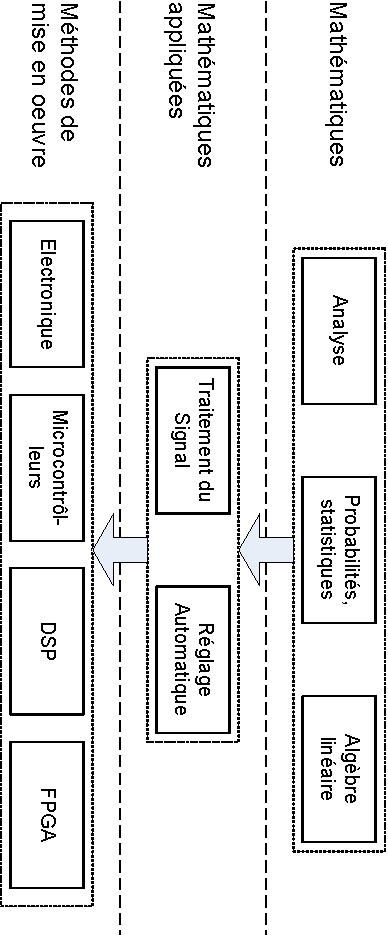
\includegraphics[angle=90, width=14cm]{./Figures/Branches.pdf}
  \rule{35em}{0.5pt}
  \caption[Situation]{Situation du cours MicroInfo dans le cursus de l'ingénieur}
  \label{fig:Branches}
\end{figure}


\section{Définitions: processeur, microprocesseur, microcontrôleur et système-on-chip}

Un processeur est un système qui permet l'exécution d'opérations élémentaires telles que des opérations arithmétiques (additions, soustractions, multiplication et division), des opérations logiques (OR, AND, XOR), des tests (égal à, plus petit que, etc.) et des déplacements de données.

Le microprocesseur est un système micro-électronique, aussi appelé circuit intégré ou plus communément "chip" ou "puce", permettant l'exécution d'opérations élémentaires. Contrairement au processeur qui est un concept, le microprocesseur est un composant que l'on place sur un circuit imprimé.

Un microcontrôleur est un système micro-électronique contenant un microprocesseur et des périphériques. Les périphériques essentiels sont les minuteries (ou "timers"), les interfaces de communication série et les mémoires (données et instructions).

Le système-on-chip est un ensemble, différent du microcontrôleur, qui inclut tous les composants électroniques d'un ordinateur à part les mémoires. Il se présente sous la forme d'un circuit intégré. La mémoire de données peut dans certain cas être assemblée en dessus du chip pour réduire la taille du système.


\section{Éléments de systèmes logiques}

Pour pouvoir configurer un microcontrôleur de manière efficace, nous avons besoins de quelques éléments de systèmes logiques.

\subsection{Définitions}

\textbf{Etat logique} : chacune des 2 valeurs que peut prendre une variable logique\\
\textbf{Variable logique} : grandeur qui ne peut prendre que les 2 états logiques\\
\textbf{Fonction logique} : variable logique qui dépend d'autres variables\\
\textbf{Table de vérité}: Liste des valeurs de sortie en fonction des combinaisons des entrées

\begin{table}[!htbp]
\begin{center}
{\fontfamily{phv}\selectfont
\begin{tabular}{|>{\centering}p{.6cm}|c|*{1}{|c}|}
\hline 
\multicolumn{2}{|c|}{Variables} & \multicolumn{1}{|c|}{Sortie}\\
\hline 
A & B & S\\
\hline  
\hline 
0 & 0 & 0\\
\hline 
0 & 1 & 0\\
\hline
1 & 0 & 0\\
\hline
1 & 1 & 1\\
\hline
\end{tabular}
}
\end{center}
\caption{Exemple de table de vérité à deux variables (fonction ET) \label{table vérité}}
\end{table}

La table de vérité permet de déterminer l'équation logique. Dans l'exemple ci dessus nous avons représenté la fonction A ET B = S. Pour construire une table de vérité on procède de la façon suivante: 
\begin{enumerate}
\item on attribue une colonne pour chaque variable ou entrée (A B C ...)
\item on attribue une colonne pour chaque résultat ou sortie
\item on liste toutes les combinaisons des variables d'entrée ($2^n$ combinaisons)
\item on calcule le résultat pour chaque ligne
\end{enumerate}

\subsection{Fonctions logiques}
Si le nombre de variables d'entrée n'est pas trop grand, on peut faire l'inventaire exhaustif de toutes les fonctions imaginables (Table \ref{variable_logiques}).

\begin{table}[!htbp]
\begin{center}
%\begin{tabular}{|p{.5cm}|c||c|c|c|c|c|c|c|c|c|c|c|c|c|c|c|c|}
{\fontfamily{phv}\selectfont
%\begin{tabular}{|c|c|*{16}{|c}|}
\begin{tabular}{|>{\centering}p{.6cm}|c|*{16}{|c}|}
\hline 
\multicolumn{2}{|c|}{Variables} & \multicolumn{16}{|c|}{Fonctions}\\
\hline 
A & B & F0 & F1 & F2 & F3 & F4 & F5 & F6 & F7 & F8 & F9 & F10 & F11 & F12 & F13 & F14 & F15\\
\hline  
\hline 
0 & 0 & 0 & 0 & 0 & 0 & 0 & 0 & 0 & 0 & 1 & 1 & 1 & 1 & 1 & 1 & 1 & 1\\
\hline 
0 & 1 & 0 & 0 & 0 & 0 & 1 & 1 & 1 & 1 & 0 & 0 & 0 & 0 & 1 & 1 & 1 & 1\\
\hline
1 & 0 & 0 & 0 & 1 & 1 & 0 & 0 & 1 & 1 & 0 & 0 & 1 & 1 & 0 & 0 & 1 & 1\\
\hline
1 & 1 & 0 & 1 & 0 & 1 & 0 & 1 & 0 & 1 & 0 & 1 & 0 & 1 & 0 & 1 & 0 & 1\\
\hline
\end{tabular}
}
$\begin{array}{rclrclcl} \\
F0&=& 0 & \quad F15&=&\overline{F0}&=&1 \\ 
F1&=&A\cdot B & \quad F14&=&\overline{F1}&=&\overline{A \cdot B} \\
F2&=&A \cdot \overline{B} & \quad F13&=&\overline{F2}&=&\overline{A}+B  \\
F3&=&A & \quad F12&=&\overline{F3}&=&\overline{A}  \\
F4&=&\overline{A} \cdot B & \quad F11&=&\overline{F4}&=&A + \overline{B} \\
F5&=&B & \quad F10&=&\overline{F5}&=&\overline{B} \\
F6&=&A \oplus B & \quad F9&=&\overline{F6}&=&\overline{A \oplus B} \\
F7&=&A+B & \quad F8&=&\overline{F7}&=&\overline{A+B} 
\end{array}$
\end{center}

\caption{Résultats possibles de fonctions à deux variables \label{variable_logiques}}
\end{table}

Dans le tableau \ref{variable_logiques}, on peut repérer trois fonctions particulières :
\begin{enumerate}
\item inversion;
\item fonction dans laquelle une seule configuration des entrées donne 1;
\item fonction dans laquelle une seule configuration des entrées donne 0.
\end{enumerate}

\subsection{Opérateurs élémentaires}

Il y a trois fonctions de base qui permettent de créer toutes les autres fonctions logiques:
\begin{center}
\begin{tabular}{p{5cm} >{\centering}p{2cm} p{3cm}} 
NON (NOT) &$\overline{A}$ &not A\\
ET (AND) &$A\cdot B$ &A and B\\
OU (OR) &$A+B$ &A or B\\
\end{tabular}
\end{center}
ET et OU sont duals, c-à-d qu'il ont des comportements semblables, mais avec les variables inverses. On peut nommer d'autres fonctions de la table 1.2 par convenance:

\begin{center}
\begin{tabular}{p{5cm} >{\centering}p{2cm} p{3cm}} 
NON ET (NAND) &$\overline{A \cdot B}$ &not(A and B)\\
NON OU (NOR) &$\overline{A+B}$ &not(A or B)\\
OU exclusif (XOR) &$A \oplus B$ &A xor B\\
NON OU exclusif (XNOR) &$\overline{A \oplus B}$ &not(A xor B)\\
\end{tabular}
\end{center}

Ces quatre fonctions supplémentaires peuvent toutes s'exprimer en fonction des trois fonctions de base. Pour les fonctions de plus de 2 variables on peut se ramener à une fonction de 2 variables par substitution. Ceci pour montrer que toute fonction logique peut se ramener aux trois fonctions de base.

\subsection{Postulats de l'algèbre de Boole}
De l'hypothèse que l'inverse d'une variable ne peut jamais avoir la même valeur que la variable, on trouve:
\begin{equation}
\begin{array}{c}
A + \overline{A} = 1 \\
A \cdot \overline{A} = 0
\end{array}
\end{equation}
Ce sont les postulats de l'algèbre de Boole.

\subsection{Théorèmes}
Grâce aux postulats nous pouvons poser une liste de théorèmes qui vont nous permettre de simplifier des équations logiques:

\begin{center}
\begin{tabular}{p{1cm} p{8cm} p{5cm}} 
1&$\overline{\overline{A}}$ &involution not(not A) = A\\
2&$A + 0=A$ &\\
3&$A \cdot 0=0$ &\\
4&$A + 1=1$ &\\
5&$A \cdot 1=A$ &\\
6&$A + A=A$ &idempotence de l'opérateur OU\\
7&$A \cdot A=A$ &idempotence de l'opérateur ET\\
8&$A + B = B + A$ &commutativité\\
9&$A \cdot B=B \cdot A$ &commutativité\\
10&$A +(B + C) = (A + B)+ C = A+B+C$ &associativité\\
11&$A \cdot (B \cdot C)= (A \cdot B) \cdot C = A\cdot B\cdot C$ &associativité\\
12&$A + B \cdot C= (A + B) \cdot (A + C)$ &distributivité\\
13&$A \cdot (B + C)= (A \cdot B) + (A \cdot C)$ &distributivité\\
14&$A \cdot B + \overline{A} \cdot B = B$ &absorption\\
15&$\overline{A + B} = \overline{A} \cdot \overline{B}$ &Théorème de De Morgan\\
16&$\overline{A \cdot B} = \overline{A} + \overline{B}$ &Théorème de De Morgan\\
17&$(A \cdot B) + (\overline{A} \cdot C) + (B \cdot C) = (A \cdot B) + (\overline{A} \cdot C)$ &Théorème du Consensus\\
18&$(A + B) \cdot (\overline{A} + C) \cdot (B + C) = (A + B) \cdot (\overline{A} + C)$ &Théorème du Consensus\\
\end{tabular}
\end{center}

\subsection{Ecriture canonique}

Définitions:
\begin{itemize}[label=\textbullet,font=\small]
\item mintermes: les lignes de la table de vérité qui donnent 1 comme résultat par fonction ET
\item maxtermes: les lignes de la table de vérité qui donnent 0 comme résultat par fonction OU
\end{itemize}

Par convention, on note $m_{x}$ le minterme tel que x est le nombre décimal égal au code binaire formé par les variables. Par exemple, $m_{5}$ est le minterme correspondant à la configuration [101] des variables d'entrée.
Par convention, on note $M_{x}$ le maxterme tel que x est le nombre décimal égal au code binaire formé par les variables. Par exemple, $M_{2}$ est le maxterme correspondant à la configuration [10] des variables d'entrée.
Une conséquence importante est que les mintermes dépendent de l'ordre dans lequel les variables sont considérées.

Pour déterminer la forme canonique d'une fonction logique dont on connait la table de vérité on peut faire la somme des mintermes:
\begin{center}
$F = m_1 + m_2 + m_3 + m_6 + m_7$
\end{center}

\begin{center}
\begin{tabular}{*{3}{|c} ||c| p{1cm} p{5cm}}
\cline{1-4} 
A & B & C & F\\
\cline{1-4}   
\cline{1-4} 
0 & 0 & 0 & 0\\
\cline{1-4} 
0 & 0 & 1 & 1 & & $\overline{A} \cdot \overline{B} \cdot C = 1$ OU\\
\cline{1-4} 
0 & 1 & 0 & 1 & & $\overline{A} \cdot B \cdot \overline{C} = 1$ OU\\
\cline{1-4} 
0 & 1 & 1 & 1 & & $\overline{A} \cdot B \cdot C = 1$ OU\\
\cline{1-4} 
1 & 0 & 0 & 0\\
\cline{1-4} 
1 & 0 & 1 & 0\\
\cline{1-4} 
1 & 1 & 0 & 1 & & $A \cdot B \cdot \overline{C} = 1$ OU\\
\cline{1-4} 
1 & 1 & 1 & 1 & & $A \cdot B \cdot C = 1$\\
\cline{1-4} 
\end{tabular}
\end{center}

\begin{center}
$F = \overline{A} \cdot \overline{B} \cdot C + \overline{A} \cdot B \cdot \overline{C} + \overline{A} \cdot B \cdot C + 
A \cdot B \cdot \overline{C} + A \cdot B \cdot C$
\end{center}

On peut aussi utiliser l'opération duale qui est le produit des maxtermes:
\begin{center}
$F = M_0 \cdot M_4 \cdot M_5$
\end{center}

\begin{center}
\begin{tabular}{*{3}{|c} ||c| p{1cm} p{5cm}}
\cline{1-4} 
A & B & C & F\\
\cline{1-4}   
\cline{1-4} 
0 & 0 & 0 & 0 & & $\overline{A} + \overline{B} + \overline{C} = 0$ ET\\
\cline{1-4} 
0 & 0 & 1 & 1\\
\cline{1-4} 
0 & 1 & 0 & 1\\
\cline{1-4} 
0 & 1 & 1 & 1\\
\cline{1-4} 
1 & 0 & 0 & 0 & & $A + \overline{B} + \overline{C} = 0$ ET\\
\cline{1-4} 
1 & 0 & 1 & 0 & & $A + \overline{B} + C = 0$\\
\cline{1-4} 
1 & 1 & 0 & 1\\
\cline{1-4} 
1 & 1 & 1 & 1\\
\cline{1-4} 
\end{tabular}\\
\end{center}

\begin{center}
$F = (\overline{A} + \overline{B} + \overline{C}) \cdot (A + \overline{B} + \overline{C}) \cdot (A + \overline{B} + C)$
\end{center}

Il est aisé de montrer que la somme des mintermes est égale au produit des maxtermes. Ceci montre encore une fois la dualité des opérations logiques. On constate aussi que le nombre de maxtermes est plus petit (3) que celui des mintermes (5). Il est donc plus simple d'utiliser le produit des maxtermes dans ce cas ci.

Le nom minterme vient du fait que dans une somme de produits, seulement un terme de la somme doit être à 1 pour donner un résultat de 1. Au contraire, dans un produit de sommes, il faut que toutes les sommes soient à 1 et donc on l'appelle maxterme.

La forme canonique est rarement optimale, il faut donc la simplifier si on cherche à optimiser l'implémentation de la fonction. Il existe des méthodes manuelles et des méthodes algorithmiques. On utilisera la méthode des tables de Karnaugh pour une réduction manuelle si le nombre de variables est limité. Au delà de 4 variables on a intérêt à utiliser une méthode algorithmique telle que celle de Quine-McCluskey.

\subsection{Opérateurs logiques en C}

La programmation des microcontrôleurs s'effectue principalement en C (2016). Nous avons donc besoin de savoir comment les opérations logiques sont représentées dans ce langage. En C, on différentie la logique sur 1 bit appelée "bit à bit" de celle sur un mot complet (8-16-32 bits). En effet, les deux types produisent des résultats différents car le FAUX sur un mot est bien '00000000' par exemple mais le VRAI comprend toutes les autres valeurs.


\begin{table}[!htbp]
\begin{center}
\begin{tabular}{|c|c|c|c|}
\hline
Opérateur & Signification & Notation C & Utilisation typique\\
\hline
AND & ET & \& & Forçage à 0 d'un bit dans un registre\\
OR & OU & | & Forçage à 1 d'un bit dans un registre\\
XOR & OU exclusif & \^{} & Inversion d'un bit dans un registre\\
NOT & inversion & $\sim$ & Inversion de tous les bits d'un registre\\
\hline
\end{tabular}
\end{center}
\caption{Opérateurs logiques bit à bit en C}
\end{table}

Exemple: 
\lstset{style=customc}
\begin{lstlisting}
char REG;
REG &= 0x7F; //force à 0 le bit no 7
\end{lstlisting}

\begin{table}[!htbp]
\begin{center}
\begin{tabular}{|c|c|c|c|}
\hline
Opérateur & Signification & Notation C & Utilisation typique\\
\hline
AND & ET & \&\& & Test logique\\
OR & OU & || & Test logique\\
NOT & négation & ! & Test logique\\
 & équivalence & == & Test logique\\
\hline
\end{tabular}
\end{center}
\caption{Opérateurs logiques booléens en C}
\end{table}

Exemple: 
\lstset{style=customc}
\begin{lstlisting}
if (REG == 0x0F)
	printf("REG est égal à 0x0F\n");
\end{lstlisting}

Les opérateurs bit à bit s'utilisent souvent pour la configuration de registres dans les microcontrôleurs, exemple:

\lstset{style=customc}
\begin{lstlisting}
REG = P1IN & (BIT5 | BIT2);
\end{lstlisting}

Les opérateurs booléens quand à eux s'utilisent surtout dans la simplification d'expressions, exemple:

\lstset{style=customc}
\begin{lstlisting}
if (!(!x && !y)) est équivalent à if (x || y)
\end{lstlisting}

%\begin{thebibliography}{1}
%
%\bibitem[1]{decoulon}Frédéric de Coulon, \emph{Théorie et traitement des signaux}, Presses polytechniques romandes, 1990
%
%\bibitem[2]{proakis}John G. Proakis, Dimitris G. Manolakis: \emph{Digital Signal Processing}, Pearson Prentice Hall, 2007
%
%\end{thebibliography}
